\let\negmedspace\undefined
\let\negthickspace\undefined
\documentclass[journal]{IEEEtran}
\usepackage[a5paper, margin=10mm, onecolumn]{geometry}
\usepackage{tfrupee} 
\setlength{\headheight}{1cm} 
\setlength{\headsep}{0mm}     

\usepackage{gvv-book}
\usepackage{gvv}
\usepackage{cite}
\usepackage{amsmath,amssymb,amsfonts,amsthm}
\usepackage{algorithmic}
\usepackage{graphicx}
\usepackage{textcomp}
\usepackage{xcolor}
\usepackage{txfonts}
\usepackage{listings}
\usepackage{enumitem}
\usepackage{mathtools}
\usepackage{gensymb}
%\usepackage{wasysym}
\usepackage{comment}
\usepackage[breaklinks=true]{hyperref}
\usepackage{tkz-euclide} 
\usepackage{listings}
\def\inputGnumericTable{}                                 
\usepackage[latin1]{inputenc}                                
\usepackage{color}                                            
\usepackage{array}                                            
\usepackage{longtable}                                       
\usepackage{calc}                                             
\usepackage{multirow}                                         
\usepackage{hhline}                                           
\usepackage{ifthen}                                           
\usepackage{lscape}
\usepackage{circuitikz}
\tikzstyle{block} = [rectangle, draw, fill=blue!20, 
    text width=4em, text centered, rounded corners, minimum height=3em]
\tikzstyle{sum} = [draw, fill=blue!10, circle, minimum size=1cm, node distance=1.5cm]
\tikzstyle{input} = [coordinate]
\tikzstyle{output} = [coordinate]
\renewcommand{\thefigure}{\theenumi}
\renewcommand{\thetable}{\theenumi}
\setlength{\intextsep}{10pt} % Space between text and floats
\numberwithin{equation}{enumi}
\numberwithin{figure}{enumi}
\renewcommand{\thetable}{\theenumi}

\begin{document}

\bibliographystyle{IEEEtran}
\vspace{3cm}

\title{12.150}
\author{EE25BTECH11032 - Kartik Lahoti}
\maketitle

\subsection*{Question: } 
Two sides of a triangle are represented by vectors $\vec{a} = \hat{i}+\hat{j}+\hat{k}$ and 
$\vec{b} = \hat{-i}+\hat{-j}+\hat{k}$. The area (magnitude) of the triangle is

\begin{enumerate}
    \begin{multicols}{4}
    \item $\frac{1}{\sqrt{2}}$
    \item $1$
    \item $\sqrt{2}$
    \item $2\sqrt{2}$
    \end{multicols}
\end{enumerate}

\textbf{Solution}:\\

Given , 
\begin{align}
    \vec{a} = \myvec{1\\1\\1} , \quad \vec{b} = \myvec{-1\\-1\\1}
\end{align}

Area of Trianle 

\begin{align}
    \frac{1}{2}\norm{\vec{a}\times\vec{b}}
\end{align}

Also, 

\begin{align}
    \vec{a}\times\vec{b} &= \myvec{\mydet{\vec{a}_{23} \quad \vec{b}_{23}} \\ \mydet{\vec{a}_{31} \quad \vec{b}_{31}} \\ \mydet{\vec{a}_{12} \quad \vec{b}_{12}}}
\end{align}

\begin{align}
    &= \myvec{1\cdot1 - 1\cdot\brak{-1} \\ 1\cdot\brak{-1} - 1\cdot1 \\ 1\cdot\brak{-1} - 1\cdot\brak{-1}} = \myvec{2\\-2\\0}
\end{align}

\begin{align}
    Ar\brak{\Delta} &= \frac{1}{2}\norm{\myvec{2\\-2\\0}}\\
                    &= \frac{1}{2}2\sqrt{2}\\
                    &= \sqrt{2}
\end{align}

Hence, Answer : Option $3$

\begin{figure}[H]
    \centering
    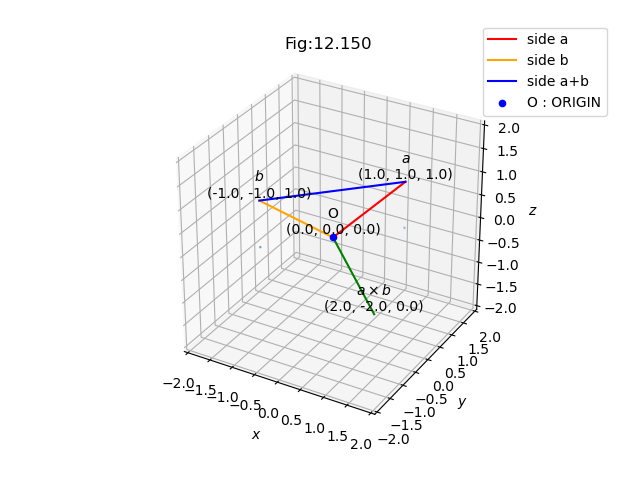
\includegraphics[width=1\columnwidth]{figs/vector2.png}
    \caption*{}
    \label{fig:placeholder}
\end{figure}

\end{document}


